\subsection{Tipo de entidad Centro}

   \begin{description}

   \item[Definición] Se refiere al objeto del mundo real: \emph{``Institución académica donde se imparten títulos universitarios''}.

   \item[Características] La entidad presenta las siguientes características:
      \begin{itemize}
         \item \textbf{Nombre:} Centro.
         \item \textbf{Tipo:} Fuerte.
         \item \textbf{Número de atributos:} 2.
         \item \textbf{Atributo/s identificador/es principal/es:} id\_centro.
         \item \textbf{Atributo/s identificador/es alternativo/s:} nombre\_centro
         \item \textbf{Atributo/s heredado/s:} -
      \end{itemize}

   \item[Diagrama] La figura \ref{diagramaCentro} muestra el diagrama de la entidad.
   \item \begin{figure}[!ht]
            \begin{center}
            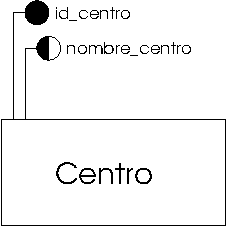
\includegraphics[]{07.Modelo_Entidad-Interrelacion/7.2.Analisis_Entidades/diagramas/centro.pdf}
            \caption{Diagrama de la entidad Centro.}
            \label{diagramaCentro}
            \end{center}
         \end{figure}

   \item[Descripción de los atributos] La entidad presenta los siguientes
   atributos:

   \begin{itemize}
    \item \textbf{id\_centro}
      \begin{itemize}
         \item \textbf{Definición:} Código que sirve como número identificativo
               para cada centro del sistema.
         \item \textbf{Dominio:} Números naturales.
         \item \textbf{Carácter:} Obligatorio.
         \item \textbf{Ejemplo práctico:} 15.
         \item \textbf{Información adicional:} El dato lo genera el sistema
               cuando el administrador principal introduce un nuevo centro en
               el sistema. Es la clave primaria.
      \end{itemize}
   \item \textbf{nombre\_centro}
      \begin{itemize}
         \item \textbf{Definición:} Denominación de un centro dentro del sistema.
         \item \textbf{Dominio:} Conjunto de caracteres alfanuméricos.
         \item \textbf{Carácter:} Obligatorio.
         \item \textbf{Ejemplo práctico:} Escuela Politécnica Superior.
         \item \textbf{Información adicional:} El dato lo introduce el
         administrador principal al introducir un nuevo centro en el sistema. Es
         clave alterna.
      \end{itemize}
   \end{itemize}

   \item[Ejemplo práctico]

   \item \begin{center}
            \begin{tabular}{ | l | l | }
            \hline
            \multicolumn{2}{ | c | }{\textbf{Tipo de entidad Centro}} \\
            \hline
            id\_centro & 15 \\
            \hline
            nombre\_centro & Escuela Politécnica Superior \\
            \hline
            \end{tabular}
         \end{center}
   \end{description}
